\documentclass[tikz,border=10pt]{standalone}
\begin{document}
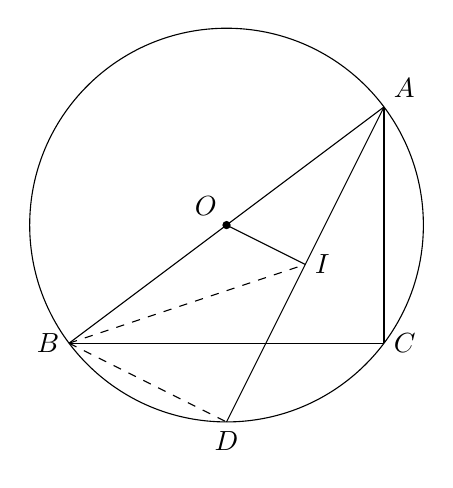
\begin{tikzpicture}
    \coordinate (O) at (0,0);
    \coordinate (A) at (2, 1.5);
    \coordinate (B) at (-2, -1.5);
    \coordinate (C) at (2, -1.5);
    \coordinate (D) at (0, -2.5);
    \coordinate (I) at (1, -0.5);

    \draw (O) circle (2.5);
    
    \draw (A) -- (B);
    \draw (A) -- (C);
    \draw (B) -- (C);
    \draw (A) -- (D);
    \draw (O) -- (I);
    
    \draw[dashed] (B) -- (I);
    \draw[dashed] (B) -- (D);
    
    \fill (O) circle (1.5pt);
    
    \node[above right] at (A) {$A$};
    \node[left] at (B) {$B$};
    \node[right] at (C) {$C$};
    \node[below] at (D) {$D$};
    \node[above left] at (O) {$O$};
    \node[right] at (I) {$I$};
\end{tikzpicture}
\end{document}
